\section{Introduction}

The Vienna Development Method (VDM)is one of the longest established
model-oriented formal methods for the development of computer-based
systems and software
\cite{Bjorner&78,Jones90a,Fitzgerald&08c}. It consists of a
group of mathematically well-founded languages for expressing system
models during early design stages, before expensive implementation
commitments are made. The construction and analysis of the model using
Overture help to identify areas of incompleteness or ambiguity in
informal system specifications, and provide some level of confidence
that a valid implementation will have key properties, especially those
of safety or security. VDM has a strong record of industrial
application, in many cases by practitioners who are not specialists in
the underlying formalism or logic
\cite{Larsen&95b,Clement&99,Kurita&09}. Experience with the method
suggests that the effort expended on formal modeling and analysis can
be recovered in reduced rework costs arising from design errors.

VDM models are expressed in a specification language (VDM-SL) that
supports the description of data and functionality
\cite{ISOVDM96a,Fitzgerald&98b,Fitzgerald&09}. Data are defined by
means of types built using constructors that define structured data
and collections such as sets, sequences and mappings from basic values
such as Booleans and numbers. These types are very abstract, allowing
the user to add any relevant constraints as data type
invariants. Functionality is defined in terms of operations over these
data types. Operations can be defined implicitly by preconditions and
postconditions that characterize their behavior, or explicitly by
means of specific algorithms. An extension of VDM-SL, called VDM++,
supports object-oriented structuring of models and permits direct
modeling of concurrency \cite{Fitzgerald&05}. An additional extension
to VDM++ is called VDM Real Time (VDM-RT) (formerly called VDM In a
Constrained Environment (VICE)) \cite{Mukherjee&00,Verhoef&06b}. All
these different dialects are supported by the unified tool called Overture.

Since the VDM modeling languages have a formal mathematical semantics,
a wide range of analyses can be performed on models, both to check
internal consistency and to confirm that models have emergent
properties. Analyses may be performed by inspection, static analysis,
testing or mathematical proof. To assist in this process, Overture
supply tool support for building models in collaboration with other
modeling tools, to execute and test models and to carry out different
forms of static analysis \cite{Larsen&10a}. It can be seen as an open
source version of the commercial tool called VDMTools
\cite{Elmstrom&94,Fitzgerald&08a} although that also have features to
generate executable code in high-level programming languages which are
not yet available in Overture.

This guide explains how to use the Overture IDE for developing models
for different VDM dialects. This user manual starts with explanantion
about how to get hold of the software in
Ssection~\ref{sec:install}. This is followed in
Section~\ref{sec:vdmsupport} with an introduction to the concepts used
in the different Overture perspectives based on Eclipse
terminology. In Section~\ref{sec:projects} it is explained how
projects are managed in the Overture IDE. In Section~\ref{sec:editVDM}
the features supported when editing VDM models are explained. This is
followed in Section~\ref{sec:debug} with an explainantion of the
interpretation and debugging capabilities in the Overture
IDE. Section~\ref{sec:testcoverage} then illustates how test coverage
information can be gathered when models are interpreted. Afterwards
Section~\ref{sec:prettyprint} shows how models with and without test
coverage information can be generated to the text processing system
\LaTeX\ and automatically converted to \texttt{pdf} format if one have
\texttt{pdflatex} installed on the computer. Afterwards from
Section~\ref{sec:POmanagement} to Section~\ref{sec:showlog} different
VDM specfic features are explained. In Section~\ref{sec:POmanagement}
the use of the notion for proof obligations and its support in
Overture is explained. In Section~\ref{sec:testing} a notion of
combinatorial testing and the automation support for that in Overture
is presented. In Section~\ref{sec:vdmuml} support for mapping between
object-oriented VDM models to and from UML models is presented. In
Section~\ref{sec:ToVDMRT} it is illustrated how one can move from a
VDM++ project to a new VDM-RT project. In Section~\ref{sec:showlog} it
is shown how support to analysing and displaying logs from executing
such VDM-RT models. After these sections the main part of the user
manual is completed in Section~\ref{sec:commandline} with an
explanantion of the features from Overture that also is available from
a command-line interface.
Finally in
Appendix~\ref{sec:index} an index of significant terms used in this
user manual can be found. 


\section{Getting Hold of the Software}\label{sec:install}

The Overture project is managed on SourceForge.  The best way to run
Overture is to download a special version of Eclipse with the Overture
functionality already pre-installed. If you go to:
  \begin{quote}
  \url{http://sourceforge.net/projects/overture/files/}
  \end{quote}
  \noindent you can find
  pre-installed versions of Overture for Windows, Linux and Mac. At a
  later stage it will also be possible to use an update site to
  install it from directly in Eclipse. However, at the moment only
  stand-alone versions are distributed because the risk of version
  problems and dependencies with other plug-ins is much smaller this way.

Zip files with a large collection of existing VDM-SL, VDM++ and VDM-RT
projects can be downloaded from
\begin{quote}
\url{http://sourceforge.net/projects/overture/files/Examples/}
\end{quote}
Such existing projects can be imported as described in
subsection~\ref{subsec:importproj}. 

\section{Using the Overture Perspective}\label{sec:vdmsupport}

\subsection{Getting into the Eclipse Terminology}

Eclipse is an open source platform based around a \emph{workbench}\index{workbench} that provides
a common look and feel to a large collection of extension products. Thus if a
user is familiar with one Eclipse product, it will generally be easy to
start using a different product on the same workbench. The Eclipse workbench consists
of several panels known as \emph{views}\index{view}, such as the Script Explorer view at the
top left of Figure~\ref{fig:userguire:OverturePerspective}. A collection of
panels is called a \emph{perspective}\index{perspective}, for example
Figure~\ref{fig:userguire:OverturePerspective} shows the standard Overture
perspective. This consists of a set of views for managing Overture projects and
viewing and editing files in a project. Different perspectives are available in
Overture as will be described later, but for the moment think about a perspective as a
useful composition of views for conducting a particular task.

\begin{figure}[!h]
\begin{center}
  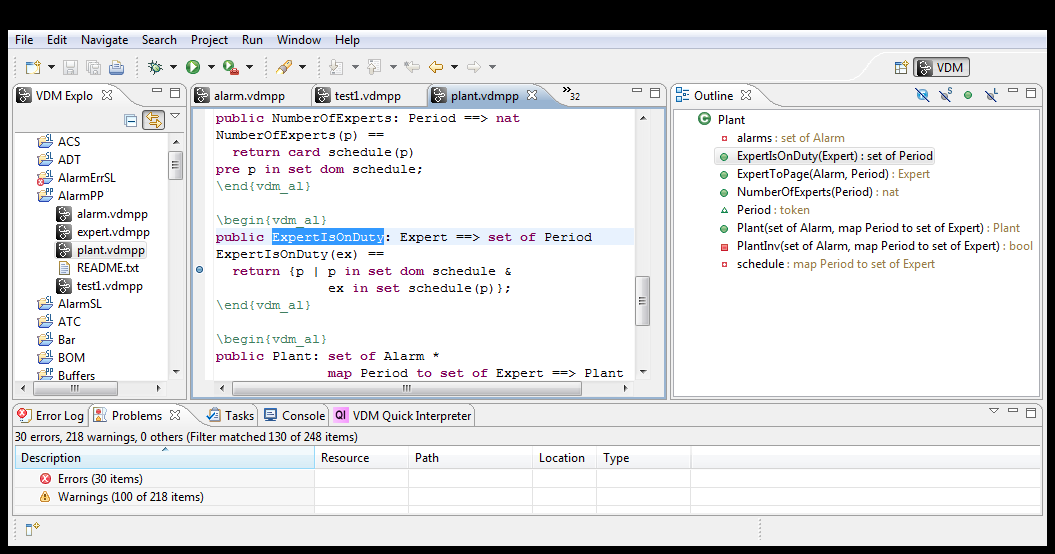
\includegraphics[width=\textwidth]{figures/OverturePerspective}
  \caption[labelInTOC]{The Overture Perspective}
  \label{fig:userguire:OverturePerspective}
\end{center}
\end{figure}

The \emph{Script Explorer view}\index{explorer} lets you create, select, and delete Overture 
projects and navigate between the files in these projects. 

Depending upon the dialect of VDM used in a given project,
a corresponding Overture editor will be available here. A new VDM-SL
project is created choosing the \emph{File} $ \rightarrow$ \emph{New}
$\rightarrow$ \emph{Project}. Then
Figure~\ref{fig:userguide:newOvertureProjectSL} will appear and \emph{Next} can
be used and then a name needs to be given to the project.


\begin{figure}[!h]
\begin{center}
  \caption[labelInTOC]{Creating a New VDM-SL Project}
  \label{fig:userguide:newOvertureProjectSL}
  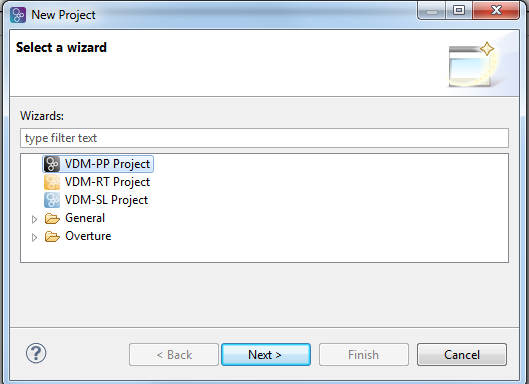
\includegraphics[width=2.5in]{figures/newovertureSLproject}
\end{center}
\end{figure}


The \emph{Outline view}\index{outline}, to the right of the editor (see
Figure~\ref{fig:userguide:OutlineView}), presents an outline of the file selected
in the editor. The outline displays any declared VDM-SL modules, as well as
their state components, values, types, functions and operations. In
case of a flat VDM-SL model the module is called {\ttfamily{DEFAULT}}.\index{DEFAULT}
% and traces.
Figure~\ref{fig:userguire:OverturePerspective} shows the outline view on the
right hand side. Clicking on an operation or function will move the cursor in
the editor to the definition of the operation. At the top of the outline view there
is a button to optionally sort what is
displayed in the outline view, for instance it is possible to hide variables.


\begin{figure}[!h]
\begin{center}
  \caption[labelInTOC]{The Outline View}
  \label{fig:userguide:OutlineView}
  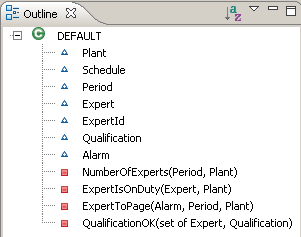
\includegraphics[width=2.5in]{figures/OutlineView}
\end{center}
\end{figure}

The \emph{Problems view}\index{problems} gathers information messages about the projects you are
working on. This includes information generated by Overture, such as
warnings and errors.

Most of the other features of the workbench, such as the menus and
toolbars, are similar to other Eclipse applications, though note that
there is a special menu with Overture specific functionality. One
convenient feature is a toolbar of shortcuts to switch between
different perspectives that appears on the right side of the screen;
these vary dynamically according to context and history.

\subsection{Additional Eclipse Features Applicab�e in Overture}


\section{Managing Overture Projects}\label{sec:projects}

\subsection{Importing Overture Projects}\label{subsec:importproj}


\subsection{Creating a New Overture Project}
\begin{enumerate}
	\item Create a new project by choosing \emph{File}
          $\rightarrow$ \emph{New} $\rightarrow$ \emph{Project}
          $\rightarrow$ \emph{Overture}; 
	\item Select the VDM dialect you wish to use (VDM-SL, VDM-PP
          or VDM-RT);\index{VDM dialect}
        \item Type in a project name
	\item Chose whether you would like the contents of the new
          project to be in your workspace or outside from existing
          source files and
        \item click
	the finish button (see \ref{fig:CreateProjectWizard}).
\end{enumerate}

\begin{figure}[!h]
	\begin{center}
	  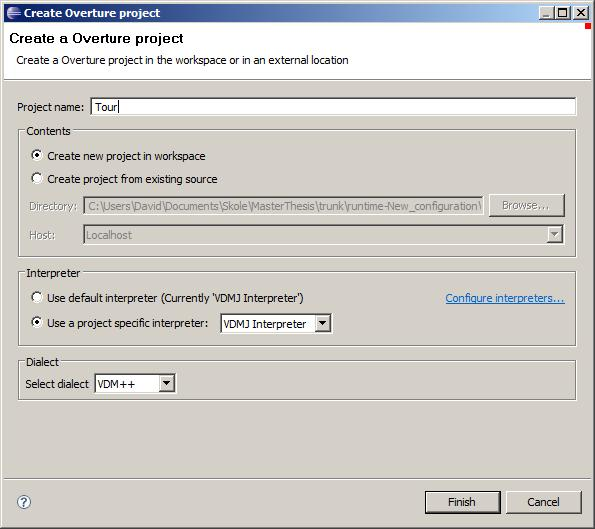
\includegraphics[scale=0.8]{figures/CreateProjectWizard}
	  \caption[Create Project Wizard]{Create Project Wizard}
	  \label{fig:CreateProjectWizard}
	\end{center}
\end{figure}

%%%%%%%%%%%%%%%%%%%%%%%%%%%%%%%%%%
%  Creating a new file
%%%%%%%%%%%%%%%%%%%%%%%%%%%%%%%%%%

\subsection{Creating Files}

Switching to the Overture perspective will change the layout of the user
interface to focus on the VDM development. To change perspective go to the menu 
window $\rightarrow$ open perspective $\rightarrow$ other\ldots and choose the
Overture perspective.
When the developer is in the Overture Perspective the user can create files
using one of the following methods:

\begin{enumerate}
  \item Choose \emph{File} $\rightarrow$ \emph{New} $\rightarrow$
    \emph{VDM-SL Module}\index{creating!VDM-SL module} or 
    \emph{VDM-PP Class}\index{creating!VDM++ class} or 
    \emph{VDM-RT Class}\index{creating!VDM-RT class} or
  \item Right click on the Overture project where you would like to
    add a new file and then choose \emph{New} $\rightarrow$ $\rightarrow$
    \emph{VDM-SL Module} or \emph{VDM-PP Class} or \emph{VDM-RT Class}.
\end{enumerate}

In both cases one needs to choose a file name and optionally choose a
directory if one does not want to place the file in the directory for
the chosen Overture project. Then a new file with the appropriate file
extension according to the chosen dialect will be created in the
selected directory. This file will use the appropriate module/class
template to get the user started with defining the module/class meant
to be placed in this new file. Naturally keywords for kinds of
definitions that will not be used can be deleted.

\subsection{Setting Project Options}\label{subsec:options}


\section{Editing VDM models}\label{sec:editVDM}


\section{Interpretation and Debugging in Overture}\label{sec:debug}

This section describes how to debug a model using the Overture IDE. 

\subsection{Debug configuration}

Debugging the model under development is done by creating a debug configuration
\index{debug configuration}
from the menu \emph{Run} $\rightarrow $ \emph{Debug configuration}
\ldots 
The debug
configuration dialog requires the following information as input to start the
debugger: the project name, the class, the starting operation/function and the
file containing the starting operation/function.
Figure~\ref{fig:userguide:debugConfiguration} shows a debug configuration,
clicking one of the browse buttons will open a dialog which give the user a list
of choices. The class and operation/function are chosen from the dialog with the
list of expandable classes, if the operation or function have arguments these
must be typed in manually.

\begin{figure}[htp]
\begin{center}
  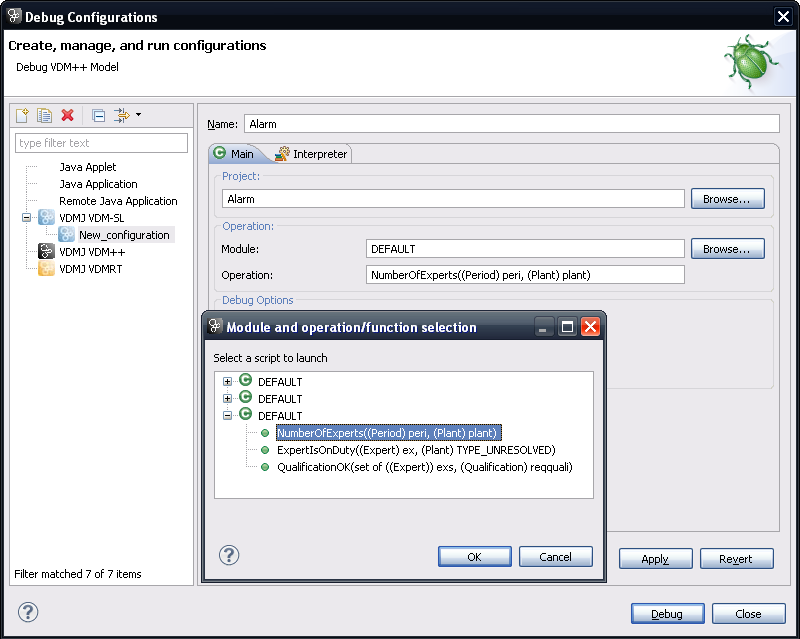
\includegraphics[width=380px]{figures/debugConfiguration}
  \caption{The debug configuration dialog}
  \label{fig:userguide:debugConfiguration}
\end{center}
\end{figure}

\subsection{Debug Perspective}

The Debug Perspective\index{debug perspective} contains the views
needed for debugging in VDM. Breakpoints can easily be set at desired
places in the model, by double clicking in left margin. When the
debugger reaches the location of the breakpoint, the user can inspect
the values of different identifiers and step through the VDM model
line by line.
 
The debug perspective shows the VDM model in an editor as the one used in the
Overture Perspective, but in this perspective there are also views useful during
debugging. The features provided in the debug perspective are described below.
The Debug Perspective is illustrated on figure~\ref{fig:userguide:DebuggingVDM}

\begin{figure}[htp]
\begin{center}
  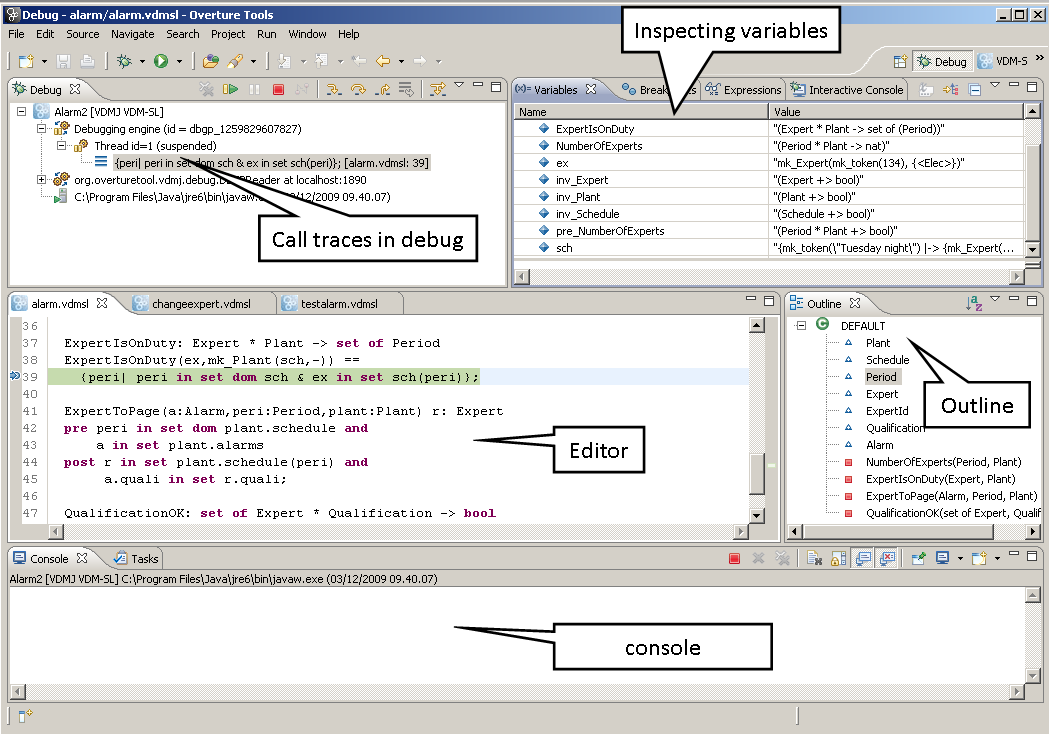
\includegraphics[width=380px]{figures/DebuggingVDM}
  \caption[Debugging perspective]{Debugging perspective}
  \label{fig:userguide:DebuggingVDM}
\end{center}
\end{figure}

The \emph{Debug view} is located in the upper left corner in the Debug
perspective. The Debug view shows all running models and the call stacks
belonging to them. It also shows whether a given model is stopped, suspended or
running. All threads are also shown, along with their running status. It is
possible to switch between threads from the Debug view.

\begin{table}
\begin{center}
\caption{Overture debugging buttons\label{tab:debugButtons}}
\begin{tabular}{|l|l|}\hline \hline
\textbf{Button} & \textbf{Explanation} \\ \hline

\includegraphics[width=0.06\textwidth]{figures/resume} & Resume
debugging\index{icon!resume debugging} \\

\includegraphics[width=0.06\textwidth]{figures/suspend} & Suspend
debugging\index{icon!suspend debugging}\\

\includegraphics[width=0.06\textwidth]{figures/terminate} & Terminate
debugging\index{icon!terminate debugging}\\

\includegraphics[width=0.06\textwidth]{figures/stepinto} & Step
into\index{icon!step into}\\

\includegraphics[width=0.06\textwidth]{figures/stepover} & Step
over\index{icon!step over} \\

\includegraphics[width=0.06\textwidth]{figures/stepreturn} & Step
return\index{icon!step return}\\

\includegraphics[width=0.06\textwidth]{figures/stepbystep} & Use step
filters\index{icon!use step filters}\\
\hline \hline
\end{tabular}
\end{center}
\end{table}

At the top of the view are buttons for controlling debugging such as; stop, step
into, step over and resume. These are standard Eclipse debugging
buttons (see Table~\ref{tab:debugButtons}).


\subsubsection{Debug View}

The debug View is located in the upper left corner in the Debug Perspective -
see figure \ref{fig:userguide:DebuggingVDM}. The debug view shows all running
models and the call stack belonging to them. It also displays whether a given model is
stopped, suspended or running. In the top of the view buttons
for debugging such as; stop, step into, step over, resume, etc.\ are located.
All threads are also shown, along with their running status. It is possible to
switch between threads from the Debug View.

\subsubsection{Variables View}
 
This view shows all the variables in a given context, when a breakpoint is
reached. The variables and their values displayed are automatically updated when
stepping through a model. The variables view is by default located in the upper
right hand corner in the Debug Perspective. It is also possible to inspect complex variables,
expanding nested arrays and so forth.

\subsubsection{Breakpoints View}

Breakpoints can be added both from the edit perspective and the debug perspective
from the editor view. In the debug perspective however, there is a breakpoints
view that shows all breakpoints. From the breakpoints view the user can easily
navigate to the location of a given breakpoint, disable, delete or set the hit
count or a break condition. In figure \ref{fig:userguide:DebuggingVDM} the
Breakpoints View is hidden behind the Variables View in the upper right hand 
corner in a tabbed notebook. Section~\ref{sec:userguide:breakpoints} explains
how to use conditional breakpoints.

\subsubsection{Expressions View}

The expressions view allows the user to write expressions, as for the
variables view, the expressions are automatically updated when stepping.
Watch expressions can be added manually or created by selecting 'create watch
expression' from the variables view. It is of course possible to edit existing
expressions. Like the Breakpoints View this view is hidden in the upper right
hand corner.

\subsubsection{Interactive Console View}

While the Expressions View allows to easily inspect values, the functionality is
somewhat limited compared with the functionality provided by VDMTools. For more
thorough inspections the Interactive Console View is more suited. Here commands
can be executed on the given context, i.e.\ where the debugger is at a
breakpoint. The Interactive console keeps a command history, so that already
executed commands can be run again without actually typing in the command all
over. Figure~\ref{fig:userguide:interactiveConsole} shows the interactive
console.

\begin{figure}[htp]
\begin{center}
  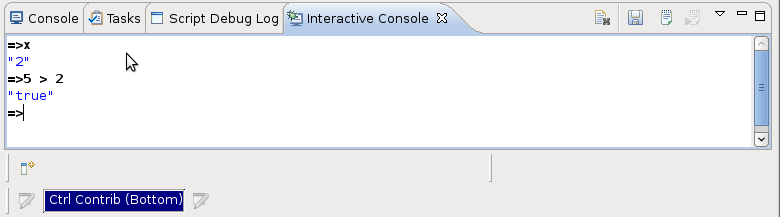
\includegraphics[width=300px]{figures/InteractiveConsole}
  \caption{The interactive console}
  \label{fig:userguide:interactiveConsole}
\end{center}
\end{figure}

\subsubsection{Conditional breakpoints}
\label{sec:userguide:breakpoints}

Conditional breakpoints can also be defined. These are a powerful tool for the
developer since it allows specifying a condition for one or more variables which
has to be true in order for the debugger to stop at the given breakpoint. Apart
from specifying a break condition depending on variables, a hit count can also be
defined. A conditional breakpoint with a hit count lets the user specify a given
number of calls to a particular place at which the debugger should break.

Making a breakpoint conditional is done by right clicking on the breakpoint
mark in the left margin and select the option Breakpoint properties\ldots This
opens a dialog like the one shown in
figure~\ref{fig:userguide:BreakpointConditional}. It is possible to choose
between two different conditional breakpoints, a hit count condition and one
based on an expression defined by the user. 

\begin{figure}[htp]
\begin{center}
  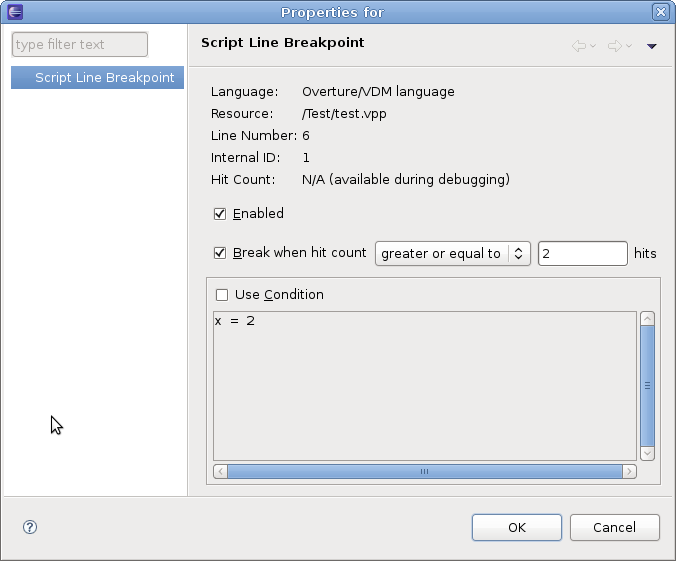
\includegraphics[width=250px]{figures/Breakpointconditional}
  \caption{Conditional breakpoint options}
  \label{fig:userguide:BreakpointConditional}
\end{center}
\end{figure}

\section{Collecting Test Coverage Information}\label{sec:testcoverage}


\section{Pretty Printing to \LaTeX}\label{sec:prettyprint}

\section{Managing Proof Obligations}\label{sec:POmanagement}


\section{Combinatorial Testing}\label{sec:testing}

In order to automate parts of the testing process a notion of
\emph{traces} have been introduced into VDM++ (note that this is not
yet available for VDM-SL models). Such traces conceptually correspond
to regular expressions that can be expanded to a collection of test
cases. Each such test case is then composed as a sequence of operation
calls. If a user defines such traces it is possible to make use of a
special combinatorial testing perspective that enables the automatic
unfolding of the traces and automatic execution of each of the test
cases. Subsequently the results of running all these can be inspected
and test cases that have detected errors in the VDM++ model can easily
be found and the user can then fix the problem and reuse the same
traces definitions.

\subsection{The Use of the Trace Definition Syntax}\label{sec:syntax}

The syntax for trace definitions are defined as:

\Rule{traces definitions}{\Lop{traces},
   \SeqPt{\Ruleref{named trace}}
}

\Rule{named trace}{\Ruleref{identifier},
  \SeqPt{\Lit{/}, \Ruleref{identifier}},
  \Lit{:},\Ruleref{trace definition list}
}

The naming of trace definitions (with the ``\texttt{/}'' separator) 
is used for indicating the paths
that are used for generated argument files for test cases
(\texttt{.arg}) and the corresponding result files
(\texttt{.res})\footnote{Currently the full path names are however
  not supported in an Overture context but this is envisaged in the future.}.

\Rule{trace definition list}{
  \Ruleref{trace definition term}, 
  \SeqPt{\Lit{;}, \Ruleref{trace definition term}}
}

So the ``\texttt{;}'' operator is used for indicating a sequencing
relationship between its \emph{trace definition term}'s.

\Rule{trace definition term}{
  \Ruleref{trace definition} \dsep
  \Ruleref{trace definition term}, \Lit{|}, \Ruleref{trace definition}
}

So the ``\texttt{|}'' operator is used for indicating alternative
choices between trace definitions. 

\Rule{trace definition}{
  \Ruleref{trace core definition} \dsep
  \Ruleref{trace bindings}, \Ruleref{trace core definition} \dsep
  \Ruleref{trace core definition}, \Ruleref{trace repeat pattern} \dsep
  \Ruleref{trace bindings}, \Ruleref{trace core definition}, 
  \Ruleref{trace repeat pattern}
}

Trace definitions can have different forms and combinations:

\begin{itemize}
\item Core definitions which includes application of operations and
  bracketed trace expressions.
\item Trace bindings where identifiers can be bound to values and in
  case of looseness ({\bf\ttfamily let} \emph{bind} {\bf\ttfamily in
  set} \emph{setexpr} {\bf\ttfamily in} \emph{expr}) this will
  give raise to multiple test cases generated.
\item Trace repeat patterns which are used whenever repetition is
  desired.
\end{itemize}

\Rule{trace core definition}{
  \Ruleref{trace apply expression} \dsep
  \Ruleref{trace bracketed expression}
}

\Rule{trace apply expression}{
  \Ruleref{identifier}, \Lit{.}, \Ruleref{identifier}, 
  \Lit{(}, \Ruleref{expression list}, \Lit{)}
}

Trace apply expressions are the most basic element in trace
definitions. The identifier before the ``\texttt{.}'' indicate an
object for with the operation (listed after the ``\texttt{.}'') is to
be applied with a list of arguments (the expression list inside the
brackets). Note that with the current syntax for trace definitions
apply expressions are limited to this form \texttt{instid.opid(args)} so it
is for example not at the moment possible to call an operation in the
same class directly as \texttt{opid(args)}. Nor is it possible with the
current syntax to make use of a particular operation in a superclass
in case of multiple possible ones which in VDM++ is would be written
as \texttt{instid.clid`opid(args)}. In the current version it is also
not allowed to call functions here directly, although that may be
changed at some stage in the future.

\Rule{trace repeat pattern}{
  \Lit{*} \dsep 
  \Lit{+} \dsep
  \Lit{?} \dsep
  \Lit{\{}, \Ruleref{numeric literal}, \Lit{\}} \dsep
  \Lit{\{}, \Ruleref{numeric literal}, \Lit{,} 
  \Ruleref{numeric literal}, \Lit{\}}
} 

The different kinds of repeat patterns have the following meanings:
\begin{itemize}
\item  \Lit{*} means 0 to n occurrences (n is tool specific). 
\item  \Lit{+} means 1 to n occurrences (n is tool specific). 
\item  \Lit{?} means 0 or 1 occurrences. 
\item  \Lit{\{}, n, \Lit{\}} means n occurrences.
\item  \Lit{\{}, n, \Lit{,} m \Lit{\}} means between n and m occurrences.
\end{itemize}

\Rule{trace bracketed expression}{
  \Lit{(}, \Ruleref{trace definition list}, \Lit{)}
}

\Rule{trace bindings}{
  \Ruleref{trace binding}, \SeqPt{\Ruleref{trace binding}}
}

\Rule{trace binding}{
  \Lop{let}, \Ruleref{local definitions}, 
             \SeqPt{\Lit{,}, \Ruleref{local definition}}, \Lop{in} \dsep
  \Lop{let}, \Ruleref{bind}, \Lop{in} \dsep
  \Lop{let}, \Ruleref{bind}, \Lop{be}, \Lop{st}, \Ruleref{expression}, \Lop{in}
}

\subsection{Using the Combinatorial Testing GUI}

Different icons are used to illustrate the verdict in a test
case. These are:
\begin{description}
\item[\hspace{-1.8mm}
\raisebox{-0.8mm}{
\includegraphics[width=0.03\textwidth]{icons/unknownWhiteBG.png}}:]
  This icon is used to indicate that the test case has not yet been
  executed.
\index{icon!not yet executed}
\item[\hspace{-1.8mm}
\raisebox{-0.8mm}{
\includegraphics[width=0.03\textwidth]{icons/okBigWhiteBG.png}}:] This icon is used to indicate that the test case has a pass
  verdict.\index{icon!pass verdict}
\item[\hspace{-1.8mm}
\raisebox{-0.8mm}{
\includegraphics[width=0.03\textwidth]{icons/undeterminedBigWhiteBG.png}}:] This icon is used to indicate that the test case has an inconclusive
  verdict.\index{icon!inconclusive verdict}
\item[\hspace{-1.8mm}
\raisebox{-0.8mm}{
\includegraphics[width=0.03\textwidth]{icons/faildBigWhiteBG.png}}:]
This icon is used to indicate that the test case has a fail
verdict.\index{icon!fail verdict}
\item[\hspace{-1.8mm}
\raisebox{-0.8mm}{
\includegraphics[height=10pt]{screenDumps/skippedIndication.png}}:] 
If test cases result in a run-time error other test cases with the
same prefix will be filtered away and thereby skipped by in the test
execution. The number of skipped test cases is indicated after number
of test cases for the trace definition name.\index{icon!skipped test case}
\end{description}

\section{Mapping VDM++ back and forth to UML}\label{sec:vdmuml}

\section{Moving from VDM++ to VDM-RT}\label{sec:ToVDMRT}

In the methodology for the development of distributed real-time
embedded systems using the VDM techniology there is a step where one
moves from a VDM++ model to a VDM-RT model \cite{Larsen&09b}. This
step is supported by the Overture tool suite where it is possible to
copy a VDM++ project into the starting point for a VDM-RT
project. This is done by right clicking on the VDM++ project to be
converted in this fashion in the Project Explorer view. In the menu
that comes up one then need to select the \emph{Overture Utility}
$\rightarrow$ \emph{Create Real Time Project}.\index{create real time
  project} As a consequence a new VDM-RT project is
created.\index{create!VDM-RT project} It will be called exactly the
same as the VDM++ project with \texttt{RT} appended to the project
name. Inside the project all the \texttt{vdmpp} files will instead
have the \texttt{vdmrt} extension. The original VDM++ project is not
changed at all. Thus this is simply an easy way to fast get the
starting point for a VDM-RT model developed. One then manually need to
create a {\ttfamily\bf system} with appropriate declarations of
\texttt{CPU}s and \texttt{BUS}ses.
 
\section{Analysing and Displaying Logs from VDM-RT Executions}\label{sec:showlog}
When a VDM-RT model is being executed a textual logfile is created in
a ''logs/debugconfig'' folder with the \emph{.logrt} extension. The
file name for the logfile indicates the time at which it has been
written so it is possible to store multiple of these. This logfile can be
viewed in the build-in RealTime Log Viewer,\index{RealTime Log viewer}
by double-clicking the file in the project view. The viewer enables
the user to explore system execution in various perspectives. In
Figure~\ref{fig:userguide:ArchitecturalOverview} the architectural
overview of the system is given, describing the distributed nature of
the model.\index{architecture overview}

\begin{figure}[htp]
\begin{center}
  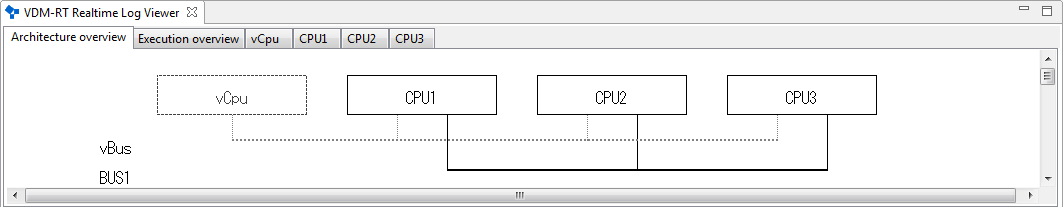
\includegraphics[width=4in]{figures/ArchitectureOverview}
  \caption{Architectural overview}
  \label{fig:userguide:ArchitecturalOverview}
\end{center}
\end{figure}

The RealTime Log Viewer also enables the user to get an overview of
the model execution\index{model execution overview} on a system level -- this can be seen in
Figure~\ref{fig:userguide:ExecutionOverview}. This view shows how the
different CPUs\index{CPU} communicate via the BUSes\index{BUS} of the system. 

\begin{figure}[htp]
\begin{center}
  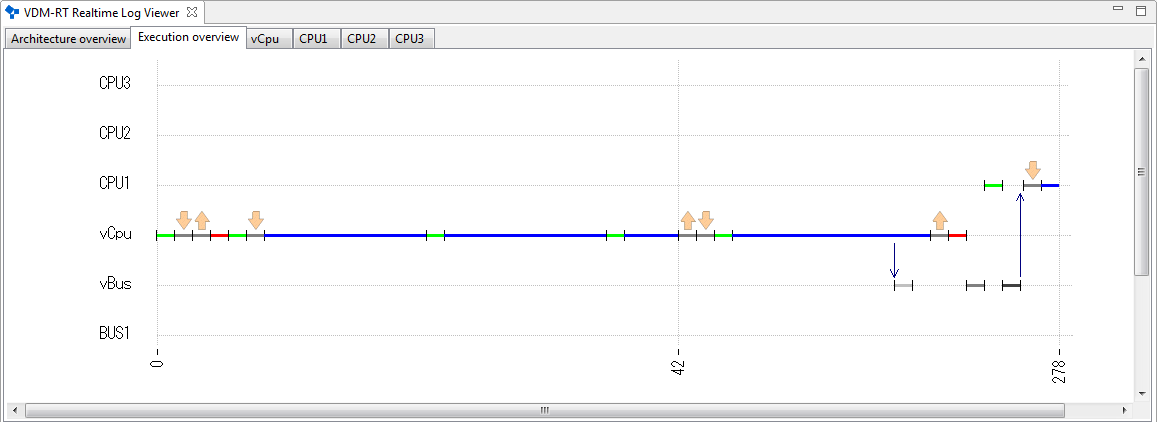
\includegraphics[width=4in]{figures/ExecutionOverview}
  \caption{Execution overview}
  \label{fig:userguide:ExecutionOverview}
\end{center}
\end{figure}

Since the complete execution of the model cannot be shown in a normal
sized window, the user has the option of jumping the a certain time
using the \emph{Go to time} button.\index{Go to time button} It is
also possible to export all the generated views to \emph{JPG} format
using the \emph{Export Image} button.\index{export image button} All
the generated pictures will be placed in the ''logs'' folder.

In addition to the execution overview, the RealTime Log Viewer can
also give an overview of all executions on a single CPU. This view
gives a detailed description of all operations and functions invoked
on the CPU as well as the scheduling of concurrent processes. This can
be seen in Figure~\ref{fig:userguide:ExecutionCPU}.\index{single CPU overview} 

\begin{figure}[htp]
\begin{center}
  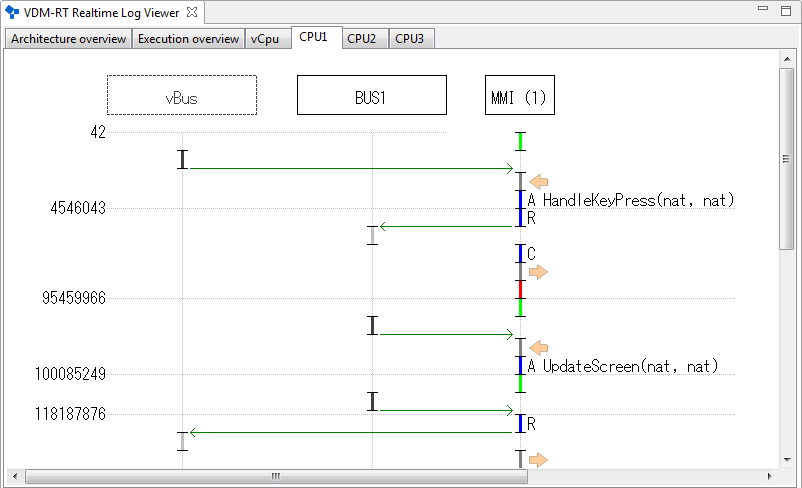
\includegraphics[width=4in]{figures/ExecutionCPU}
  \caption{Execution on single CPU}
  \label{fig:userguide:ExecutionCPU}
\end{center}
\end{figure}

\section{A Command-Line Interface to VDMJ}\label{sec:commandline}

A central part of the Overture tool is gathered in a java application
called VDMJ that enables a command-line interface that may be valuable
for users outside the Eclipse interface of Overture.

\subsection{Starting VDMJ}

VDMJ\index{VDMJ} is contained entirely within one jar file. The jar
file contains a MANIFEST that identifies the main class to start the
tool, so the minimum command line invocation is as follows:

\lstset{style=tool,language=}
\begin{lstlisting}
$ !\textbf{java -jar vdmj-2.0.0.jar}�
VDMJ: You must specify either -vdmsl, -vdmpp or -vdmrt
Usage: VDMJ <-vdmsl | -vdmpp | -vdmrt > [<options>] [<files>]
-vdmsl: parse files as VDM-SL
-vdmpp: parse files as VDM++
-vdmrt: parse files as VICE
-w: suppress warning messages
-q: suppress information messages
-i: run the interpreter if successfully type checked
-p: generate proof obligations and stop
-e <exp>: evaluate <exp> and stop
-c <charset>: select a file charset
-t <charset>: select a console charset
-o <filename>: saved type checked specification
-pre: disable precondition checks
-post: disable postcondition checks
-inv: disable type/state invariant checks
-dtc: disable all dynamic type checking
-log: enable real-time event logging
\end{lstlisting}
\lstset{style=mystyle}
\lstset{language=VDM++}

Notice that the error indicates that the tool must be invoked with either the \texttt{-vdmsl}, \texttt{-vdmpp} or \texttt{-vdmrt}
option to indicate the VDM dialect and parser required.

Normally, a specification will be loaded by identifying all of the VDM source files to include. At least
one source file must be specified unless the -i option is used, in which case the interpreter can be
started with no specification.

If no \texttt{-i} option is given, the tool will parse and type check
the specification files only, giving any errors and warnings on
standard output, then stop. Warnings can be suppressed with the \texttt{-w}
option. The \texttt{-q} option can be used to suppress the various
information messages printed (this does not include errors and
warnings).

The \texttt{-p} option will run the proof obligation generator and
then stop, assuming the specification has no type checking errors.
For batch execution, the \texttt{-e} option can be used to identify a
single expression to evaluate in the context of the loaded
specification, assuming the specification has no type checking errors.

The \texttt{-c} and \texttt{-t} options allow the file and console character sets to be defined, respectively. This is to
allow a specification written in languages other than the default for your system to be used (see
section 3).

The \texttt{-o} option allows a parsed and type checked specification to be saved to a file. Such files are
effectively libraries, and can be can be re-loaded without the parsing/checking overhead.
The \texttt{-pre}, \texttt{-post}, \texttt{-inv} and \texttt{-dtc} options can be used to disable precondition, postcondition, invariant and
dynamic type checking, respectively. By default, all these checks are performed.
The \texttt{-log} option is for use with \texttt{-vdmrt}, and causes real-time events from the model to be written to the
file name given. These are useful with the Overture Eclipse GUI, which has a plugin to display timing
diagrams [8].

If flat.vdmsl contains a simple VDM-SL specification of the factorial
function, called ``\texttt{fac}'', the following
illustrate ways to test the specification, with user input shown in bold:

\begin{lstlisting}
functions
fac: int -> int
fac(a) == if a < 2 then 1 else a * fac(a-1)
pre a > 0
\end{lstlisting}
\lstset{style=tool,language=}

\begin{lstlisting}
$ !\textbf{java -jar vdmj-2.0.0.jar -vdmsl flat.vdmsl}�
Parsed 1 module in 0.202 secs. No syntax errors
Warning 5012: Recursive function has no measure in (flat.vdmsl) at 
line 3:1
Type checked 1 module in 0.016 secs. No type errors and 1 warning
\end{lstlisting}

\begin{lstlisting}
$ !\textbf{java -jar vdmj-2.0.0.jar -vdmsl -q -w flat.vdmsl}�
<quiet!>
\end{lstlisting}

\begin{lstlisting}
$ !\textbf{java -jar vdmj-2.0.0.jar -vdmsl -w -e "fac(10)" flat.vdmsl}�
Parsed 1 module in 0.28 secs. No syntax errors
Type checked 1 module in 0.031 secs. No type errors, 
suppressed 1 warning
Initialized 1 module in 0.031 secs.
3628800
Bye
\end{lstlisting}

\begin{lstlisting}
$ !\textbf{java -jar vdmj-2.0.0.jar -vdmsl -e "fac(10)" -q -w flat.vdmsl}�
3628800
\end{lstlisting}

\begin{lstlisting}
$ !\textbf{java -jar vdmj-2.0.0.jar -vdmsl -i -w flat.vdmsl}�
Parsed 1 module in 0.202 secs. No syntax errors
Type checked 1 module in 0.016 secs. No type errors, 
suppressed 1 warning
Initialized 1 module in 0.031 secs.
Interpreter started
> !\textbf{print fac(10)}�
= 3628800
Executed in 0.0 secs.
> !\textbf{quit}�
Bye
\end{lstlisting}

\begin{lstlisting}
$ !\textbf{java -jar vdmj-2.0.0.jar -vdmsl -p -w flat.vdmsl}�
Parsed 1 module in 0.218 secs. No syntax errors
Type checked 1 module in 0.015 secs. No type errors, 
suppressed 1 warning
Generated 1 proof obligation:
Proof Obligation 1:
fac: function apply obligation in 'DEFAULT1' (flat.vdmsl) at 
line 4:38
(forall a:int & (a > 0) =>
(not (a < 2) =>
pre_f((a - 1))))
\end{lstlisting}

\begin{lstlisting}
$ !\textbf{java -jar vdmj-2.0.0.jar -vdmsl -w -e "fac(0)" -w flat.vdmsl}�
Parsed 1 module in 0.203 secs. No syntax errors
Type checked 1 module in 0.015 secs. No type errors, 
suppressed 1 warning
Initialized 1 module in 0.016 secs.
Execution: Error 4055: Precondition failure: pre_f in (flat.vdmsl) 
at line 5:11
   a = 0
   fac = (int -> int)
   pre_fac = (int +> bool)
In root context of fac(a) in 'DEFAULT1' (console) at line 1:1
In root context of interpreter in 'DEFAULT1' (flat.vdmsl) at 
line 3:1
In root context of global environment
Bye
\end{lstlisting}

\begin{lstlisting}
$ !\textbf{java -jar vdmj-2.0.0.jar -vdmsl -w -pre -e "fac(0)" 
-w flat.vdmsl}�
Parsed 1 module in 0.218 secs. No syntax errors
Type checked 1 module in 0.016 secs. No type errors, 
suppressed 1 warning
Initialized 1 module in 0.015 secs.
1
Bye
\end{lstlisting}

\begin{lstlisting}
$ !\textbf{java -jar vdmj-2.0.0.jar -vdmsl -w -o flat.lib flat.vdmsl}�
Parsed 1 module in 0.203 secs. No syntax errors
Type checked 1 module in 0.016 secs. No type errors, 
suppressed 1 warning
Saved 1 module to flat.lib in 0.093 secs.
\end{lstlisting}

\begin{lstlisting}
$ !\textbf{java -jar vdmj-2.0.0.jar -vdmsl flat.lib -e "fac(10)"}�
Loaded 1 module from flat.lib in 0.187 secs
Initialized 1 module in 0.0 secs.
3628800
Bye
\end{lstlisting}

\subsection{Parsing, Type Checking, and Proof Obligations}

All specification files loaded by VDMJ are parsed and type checked
automatically. There are no type checking options; the type checker
always uses ``possible'' semantics. If a specification does not parse
and type check cleanly, the interpreter cannot be started and proof
obligations cannot be generated (though warnings are allowed).

All warnings and error messages are printed on standard output, even
with the \texttt{-q} option.  A source file may contain VDM embedded
in a LaTeX file; the markup is ignored by the parser, though reported
line numbers will be correct.

The Java program will return with an exit code of zero if the
specification is clean (ignoring warnings).  Parser or type checking
errors result in an exit code of 1. The interpreter and PO generator
always exit with a code of zero.

\subsection{The Interpreter}

Assuming a specification does not contain any parse or type checking errors, the interpreter can be
started by using the \texttt{-i} command line option.
The interpreter is an interactive command line tool that allows expressions to be evaluated in the
context of the specification loaded. The interpreter prompt is ``\texttt{>}''. The following illustrates some of the
interactive interpreter commands (explanation below. The shmem source
model is in Appendix A):

\begin{lstlisting}
$ !\textbf{java -jar vdmj-2.0.0.jar -vdmsl -i shmem.vdmsl}�
Parsed 1 module in 0.266 secs. No syntax errors
Type checked in 0.047 secs. No type errors
Interpreter started
\end{lstlisting}

\begin{lstlisting}
> !\textbf{help}�
modules - list the loaded module names
default <module> - set the default module name
state - show the default module state
print <expression> - evaluate expression
assert <file> - run assertions from a file
init - re-initialize the global environment
env - list the global symbols in the default environment
pog - generate a list of proof obligations
break [<file>:]<line#> [<condition>] - create a breakpoint
break <function/operation> [<condition>] - create a breakpoint
trace [<file>:]<line#> [<exp>] - create a tracepoint
trace <function/operation> [<exp>] - create a tracepoint
remove <breakpoint#> - remove a trace/breakpoint
list - list breakpoints
coverage [<file>|clear] - display/clear file line coverage
latex|latexdoc [<files>] - generate LaTeX line coverage files
files - list files in the current specification
reload - reload the current specification files
load <files> - replace current loaded specification files
quit - leave the interpreter
\end{lstlisting}

\begin{lstlisting}
> !\textbf{modules}�
M (default)
\end{lstlisting}

\begin{lstlisting}
> !\textbf{state}�
M`Q4 = [mk_M(<FREE>, 0, 9999)]
M`rseed = 87654321
M`Memory = mk_Memory(87654321, [mk_M(<FREE>, 0, 9999)],
                               [mk_M(<FREE>, 0, 9999)])
M`Q3 = [mk_M(<FREE>, 0, 9999)]
\end{lstlisting}

\begin{lstlisting}
> !\textbf{print rand(100)}�
= 71
Executed in 0.0 secs.
\end{lstlisting}

\begin{lstlisting}
> !\textbf{print rand(100)}�
= 44
Executed in 0.0 secs.
\end{lstlisting}

\begin{lstlisting}
> !\textbf{state}�
M`Q4 = [mk_M(<FREE>, 0, 9999)]
M`rseed = 566044643
M`Memory = mk_Memory(566044643, [mk_M(<FREE>, 0, 9999)], 
                                [mk_M(<FREE>, 0, 9999)])
M`Q3 = [mk_M(<FREE>, 0, 9999)]
\end{lstlisting}

\begin{lstlisting}
> !\textbf{init}�
Global context initialized
\end{lstlisting}

\begin{lstlisting}
> !\textbf{state}�
M`Q4 = [mk_M(<FREE>, 0, 9999)]
M`rseed = 87654321
M`Memory = mk_Memory(87654321, [mk_M(<FREE>, 0, 9999)],
                               [mk_M(<FREE>, 0, 9999)])
M`Q3 = [mk_M(<FREE>, 0, 9999)]
\end{lstlisting}

\begin{lstlisting}
> !\textbf{print rand(100)}�
= 71
Executed in 0.0 secs.
\end{lstlisting}

\begin{lstlisting}
> !\textbf{print rand(100)}�
= 44
Executed in 0.0 secs.
\end{lstlisting}

\begin{lstlisting}
> !\textbf{env}�
M`fragments = (M`Quadrant -> nat)
M`combine = (M`Quadrant -> M`Quadrant)
M`tryBest = (nat ==> nat)
M`seed = (nat1 ==> ())
M`reset = (() ==> ())
M`bestfit = (nat1 * M`Quadrant -> nat1)
M`add = (nat1 * nat1 * M`Quadrant -> M`Quadrant)
M`firstFit = (nat1 ==> bool)
M`rand = (nat1 ==> nat1)
M`tryFirst = (nat ==> nat)
M`main = (nat1 * nat1 ==> seq of (<SAME> | <BEST> | <FIRST>))
M`MAXMEM = 10000
M`delete = (M`M * M`Quadrant -> M`Quadrant)
M`inv_M = (M`M +> bool)
M`CHUNK = 100
M`bestFit = (nat1 ==> bool)
M`least = (nat1 * nat1 -> nat1)
M`fits = (nat1 * M`Quadrant -> nat1)
M`init_Memory = (M`Memory +> bool)
M`pre_add = (nat1 * nat1 * M`Quadrant +> bool)
\end{lstlisting}

\begin{lstlisting}
> !\textbf{pog}�
Generated 36 proof obligations:
Proof Obligation 1:
M`fits: cases exhaustive obligation in 'M' (shmem.vdm) at 
line 40:5
(forall size:nat1, Q:Quadrant &
Q = [] or Q = [h] ^ tail)
...
Proof Obligation 35:
M`tryBest: sequence apply obligation in 'M' (shmem.vdm) at 
line 176:27
rand((len Q4)) in set inds Q4
Proof Obligation 36:
M`tryBest: subtype obligation in 'M' (shmem.vdm) at line 166:1
RESULT >= 0
\end{lstlisting}

This example shows a VDM-SL specification called \texttt{shmem.vdmsl} being
loaded. The help command lists the interpreter commands
available. Note that several of them regard the setting of
breakpoints, which is covered in the next section.

The modules command lists the names of the modules loaded from the
specification. In this example there is only one, called ``M''. One of
the modules is identified as the default; names in the default module
do not need to be qualified (so you can say print xyz rather than
print M`xyz). The default module can be changed with the default
command.

The state command lists the content of the default module's
state. This can be changed by operations, as can be seen by the two
calls to rand which change the rseed value in the state (a
pseudo-random number generator). The init command will re-initialize
the state to its original value, illustrated by the fact that two
subsequent calls to rand return the same results as the first two did.

The {\ttfamily{\bf print}} command can be used to evaluate any expression.
The env command lists all the values in the global environment of the default module. This shows the
functions, operations and constant values defined in the module. Note that it includes invariant,
initialization and pre/postcondition functions.
The pog command (proof obligation generator) generates a list of proof obligations for the
specification.

The assert command (illustrated below) can take a list of assertions
from a file, and execute each of them in turn, raising an error for
any assertion which is false. The assertions in the file must be
simple boolean expressions, one per line:

